\section{Appendix}
\subsection{Box Plots of Remaining Continuous Variables}
\begin{figure}[H]
    \centering
    \begin{subfigure}[b]{0.48\textwidth}
        \centering
        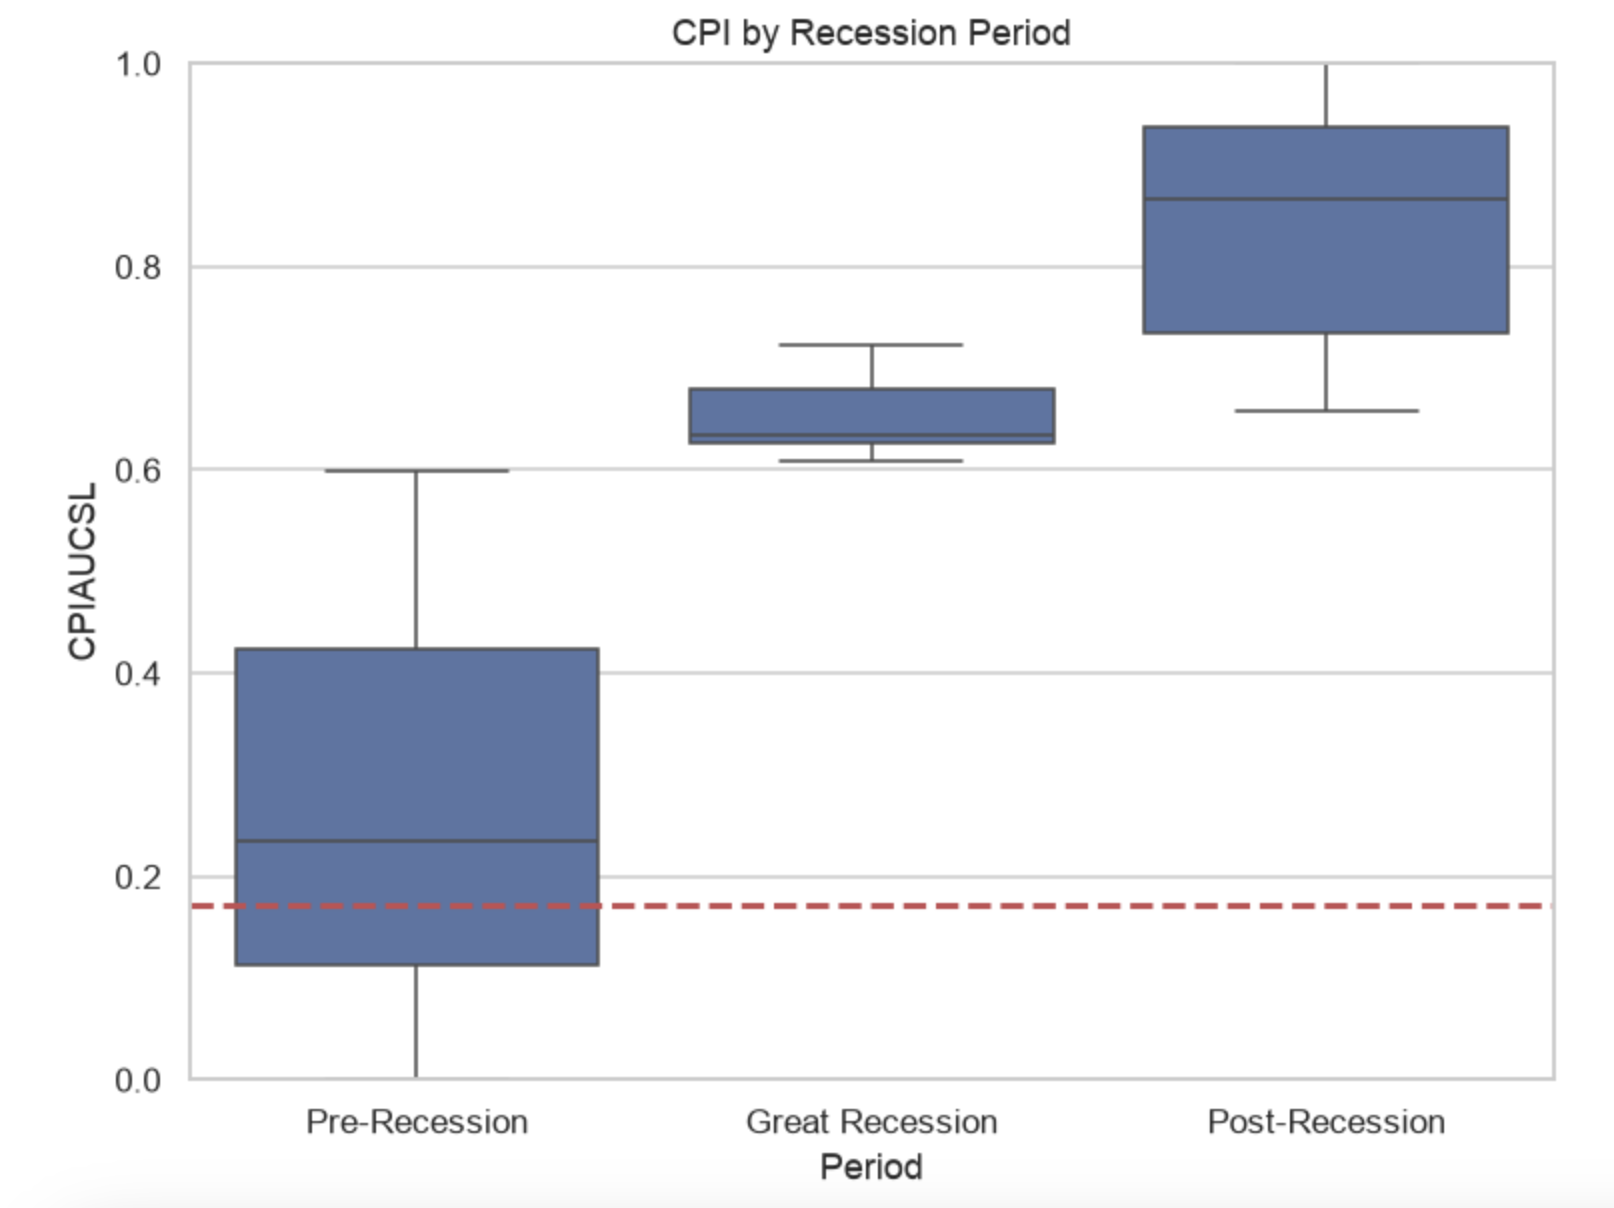
\includegraphics[width=\linewidth]{CPI boxplot.png}
        \caption{\textbf{CPI Box Plot}}
        \label{fig:cpi_box}
    \end{subfigure}
    \hfill
    \begin{subfigure}[b]{0.48\textwidth}
        \centering
        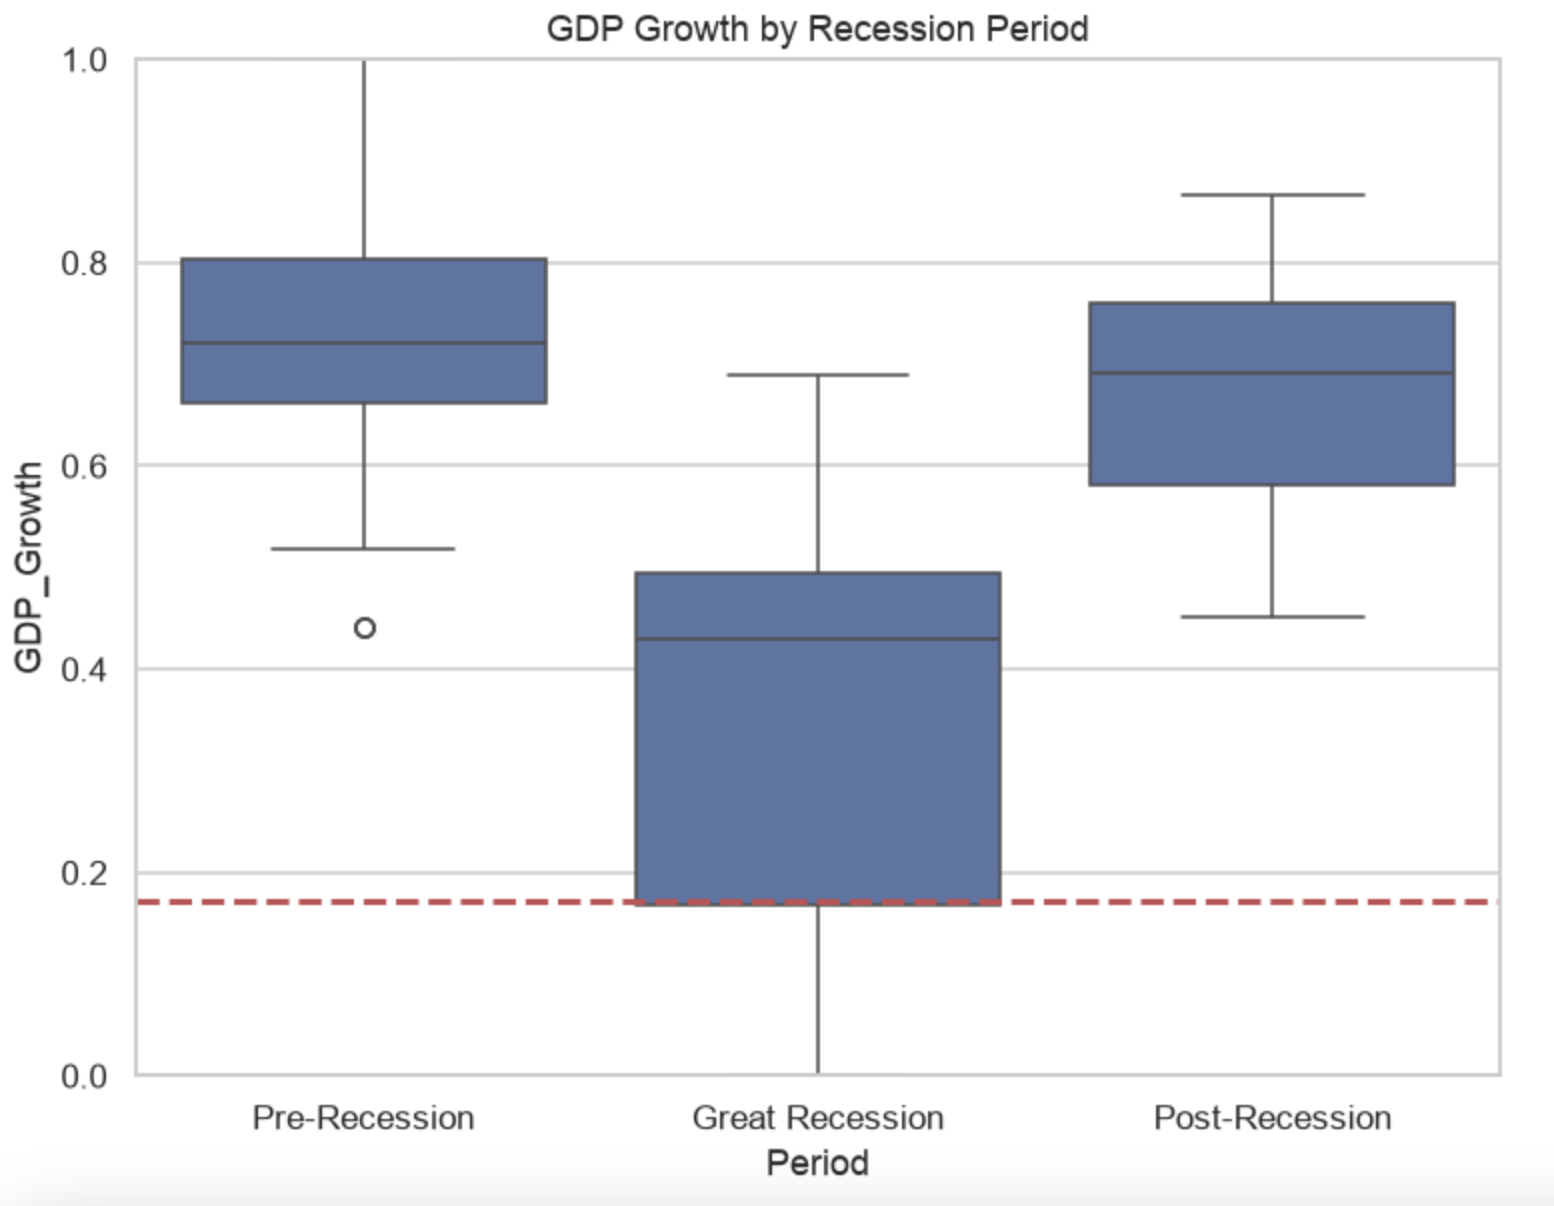
\includegraphics[width=\linewidth]{GDP boxplot.png}
        \caption{\textbf{GDP Growth Box Plot}}
        \label{fig:gdp_box}
    \end{subfigure}

    \vspace{1em}

    \begin{subfigure}[b]{0.48\textwidth}
        \centering
        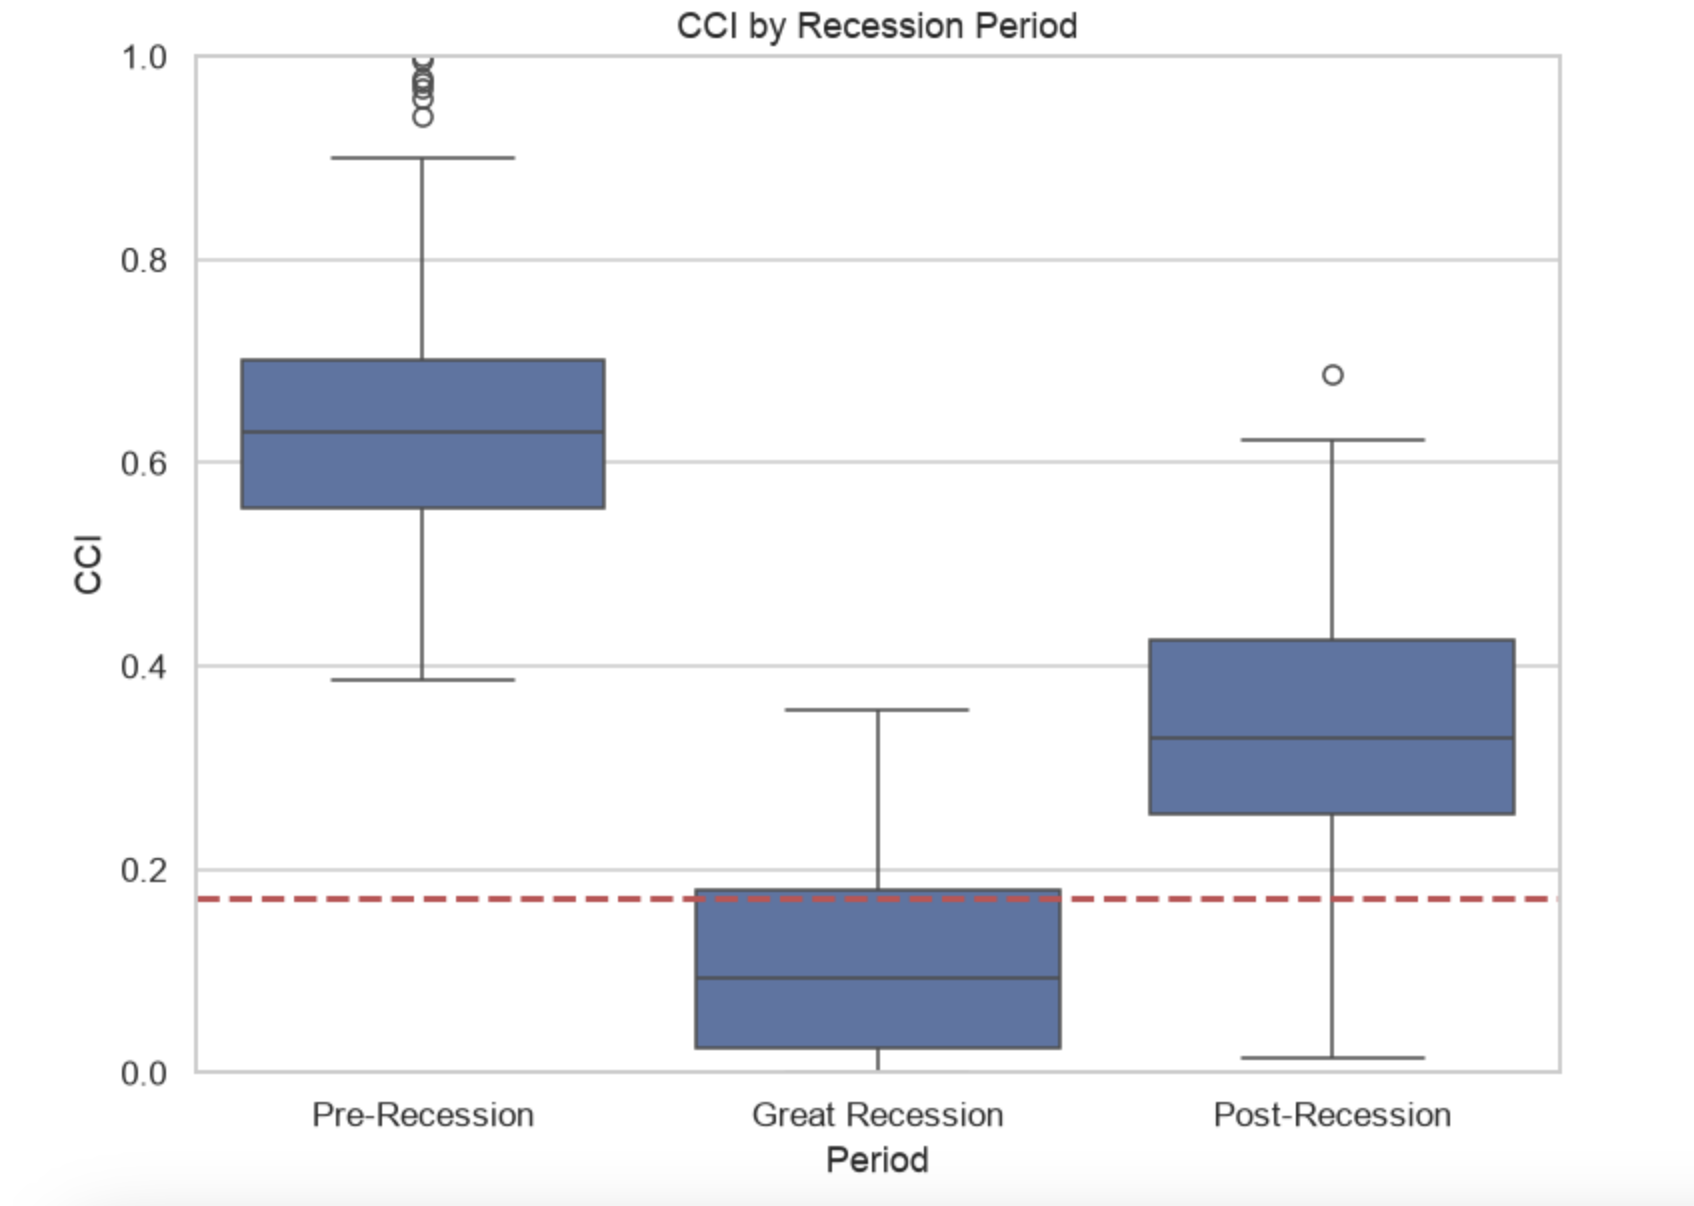
\includegraphics[width=\linewidth]{CCI Box Plot.png}
        \caption{\textbf{CCI Box Plot}}
        \label{fig:cci_box}
    \end{subfigure}

    \caption{\textbf{Box Plots by Recession Period}}
    \label{fig:boxplots}
\end{figure}
\vspace{0.8em}

\subsection{Q-Q Plots of Remaining Variables}
\begin{figure}[H]
    \centering
    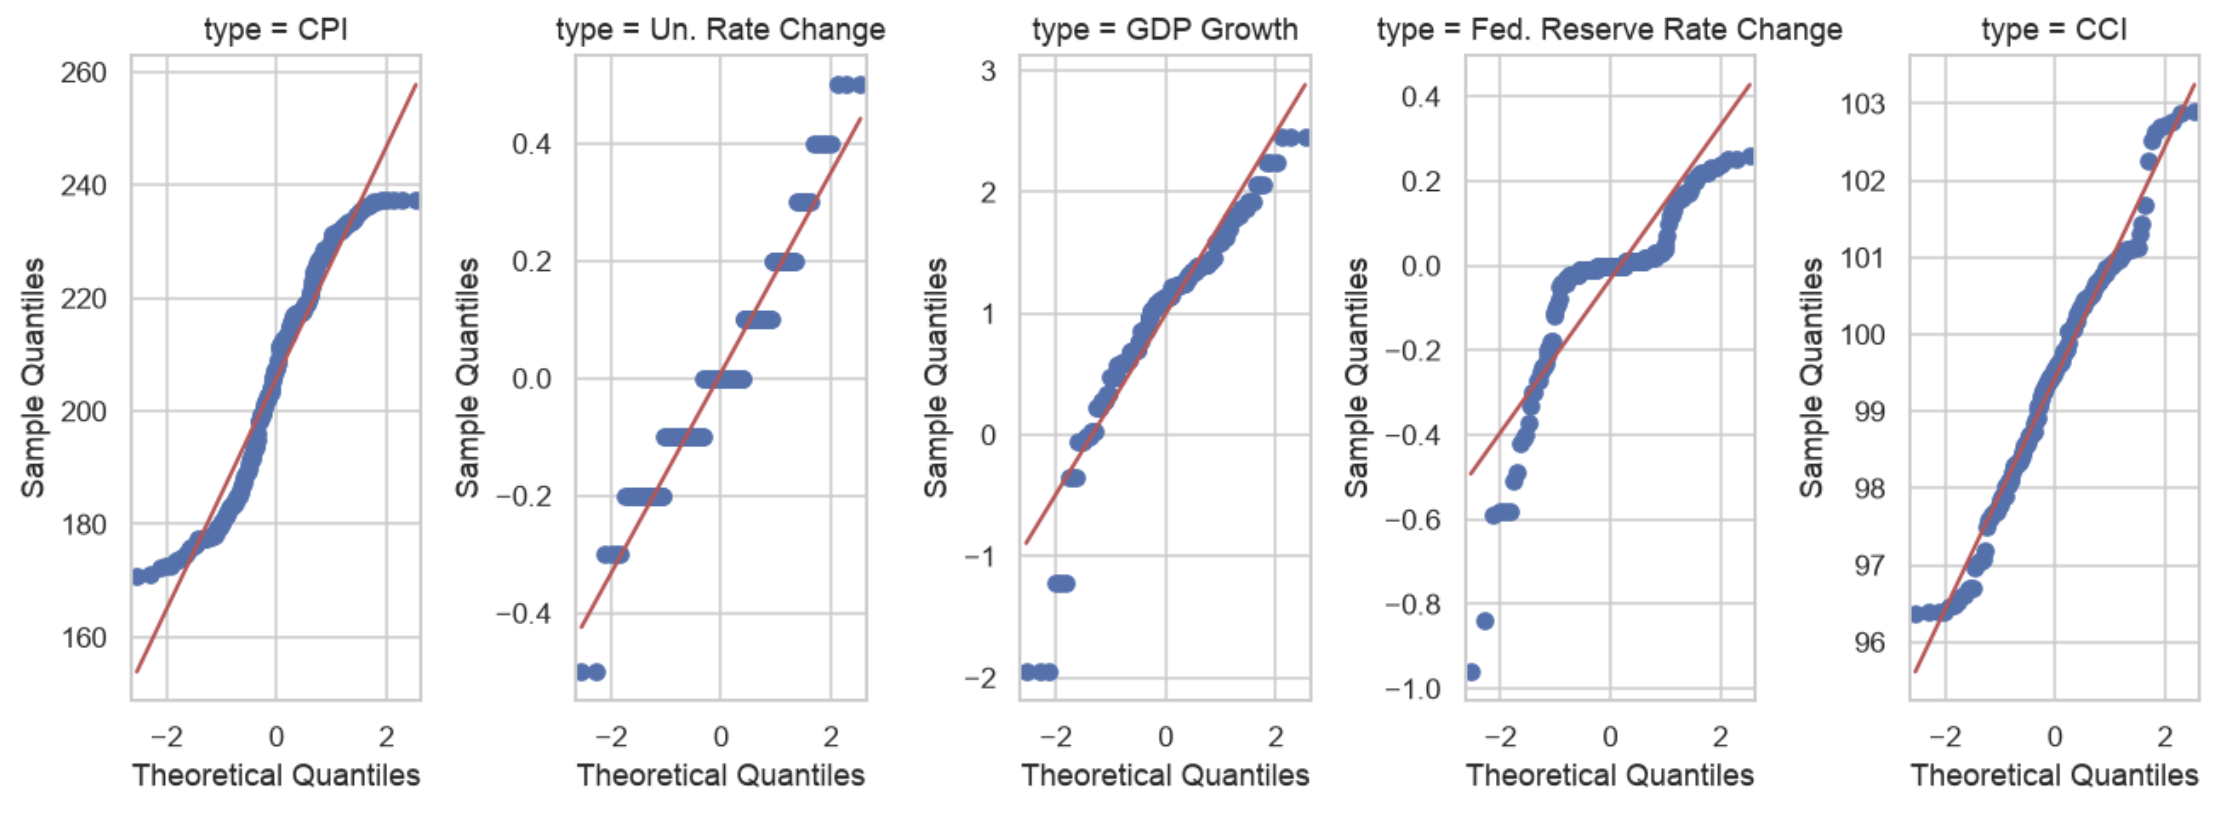
\includegraphics[width=0.75\linewidth]{Remaining QQ plots.png}
    \caption{\textbf{Q-Q Plots}}
    \label{fig:placeholder}
\end{figure}
\vspace{0.8em}
\begin{figure}[H]
    \centering
    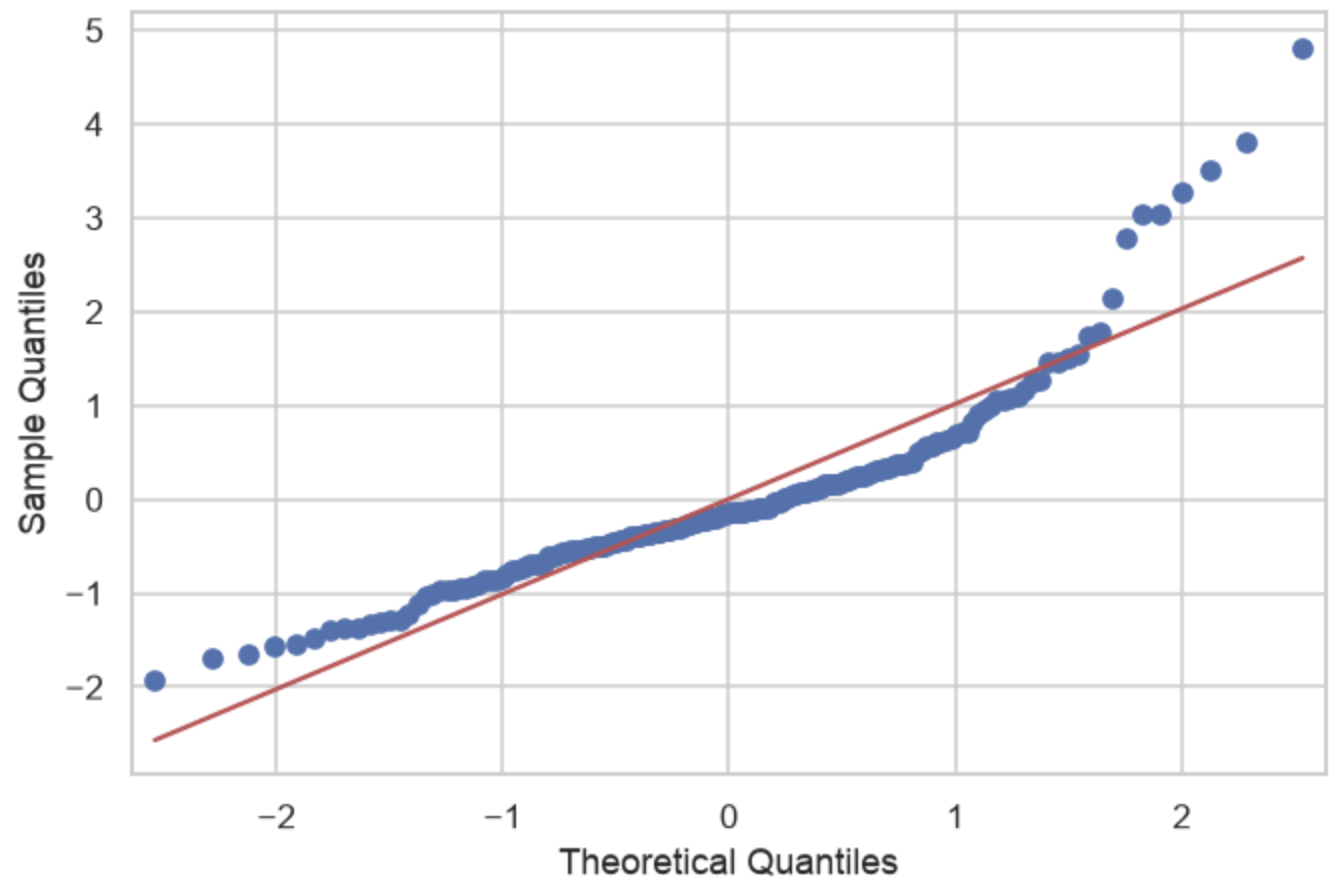
\includegraphics[width=0.5\linewidth]{QQ of standardized resid.png}
     \caption{\textbf{Q-Q Plot of Standardized Residuals}}
    \label{fig:placeholder}
\end{figure}
Figure 18 above shows the Q-Q plots of remaining predictors. The plots of Un. Rate Change and the Fed. Reserve IR Change cannot be interpreted as they are not continuous variables. All other Q-Q plots demonstrate normality, though with varying degrees. The Q-Q plot of residuals in Figure 19 show some residuals deviating from the normal distribution, at the ends. This is similar to that of the Q-Q plot of Volatility (Figure 5).

\subsection{Density Plots of Remaining Variables}
\begin{figure}[H]
    \centering
    \begin{subfigure}[b]{0.48\textwidth}
        \centering
        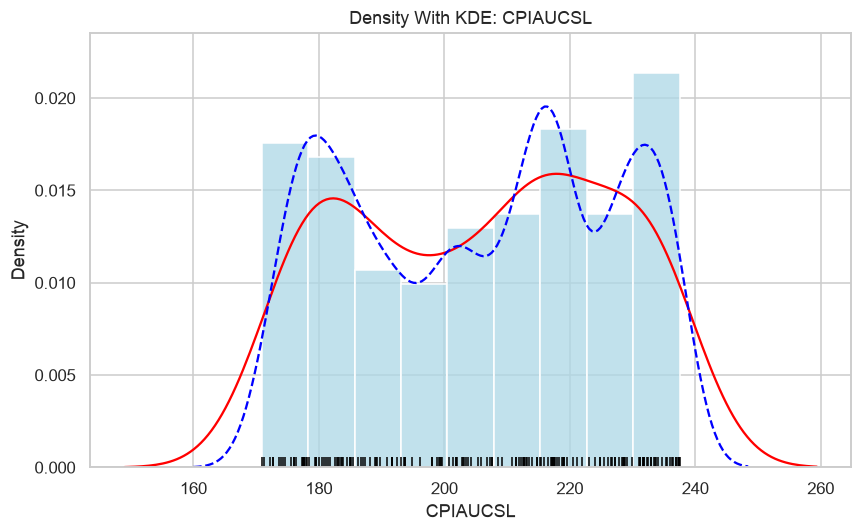
\includegraphics[width=\linewidth]{CPI density.png}
        \caption{\textbf{CPI Density}}
        \label{fig:cpi_density}
    \end{subfigure}
    \hfill
    \begin{subfigure}[b]{0.48\textwidth}
        \centering
        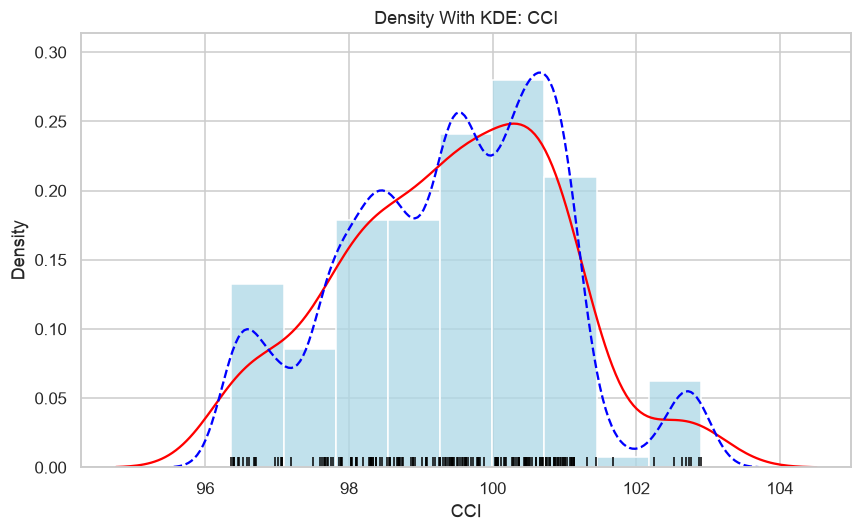
\includegraphics[width=\linewidth]{CCI Density.png}
        \caption{\textbf{CCI Density}}
        \label{fig:cci_density}
    \end{subfigure}

    \vspace{1em}

    \begin{subfigure}[b]{0.48\textwidth}
        \centering
        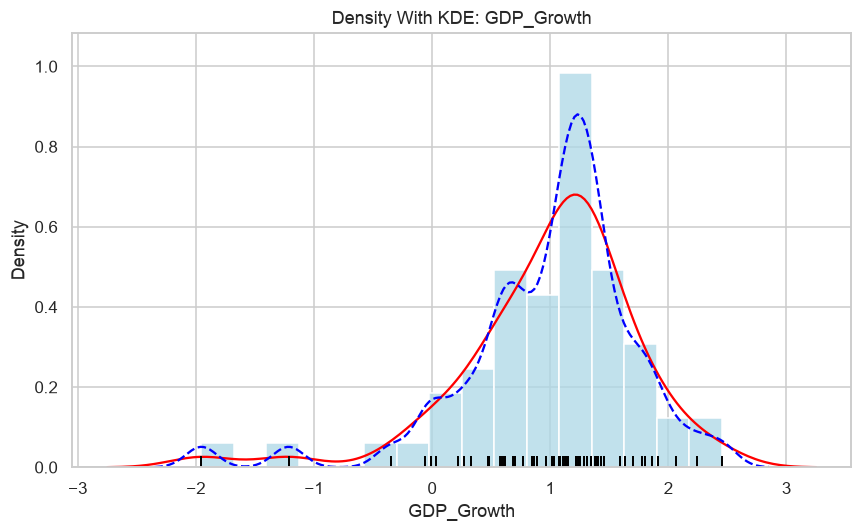
\includegraphics[width=\linewidth]{GDP Density.png}
        \caption{\textbf{GDP Growth Density}}
        \label{fig:gdp_density}
    \end{subfigure}

    \caption{\textbf{Density Plots of the Model Variables}}
    \label{fig:densities}
\end{figure}
%\input project components?